% ----------------------------- APPENDIX ------------------------------
\section{Appendix}
\label{app:diagnostics}

% Optional: slightly tighter appendix figure captions
\captionsetup[figure]{font=footnotesize,labelfont=bf,skip=4pt}

% Optional: common appendix figure width
\newcommand{\appfigwidth}{0.7\linewidth}

\begin{figure}[H]
    \centering
    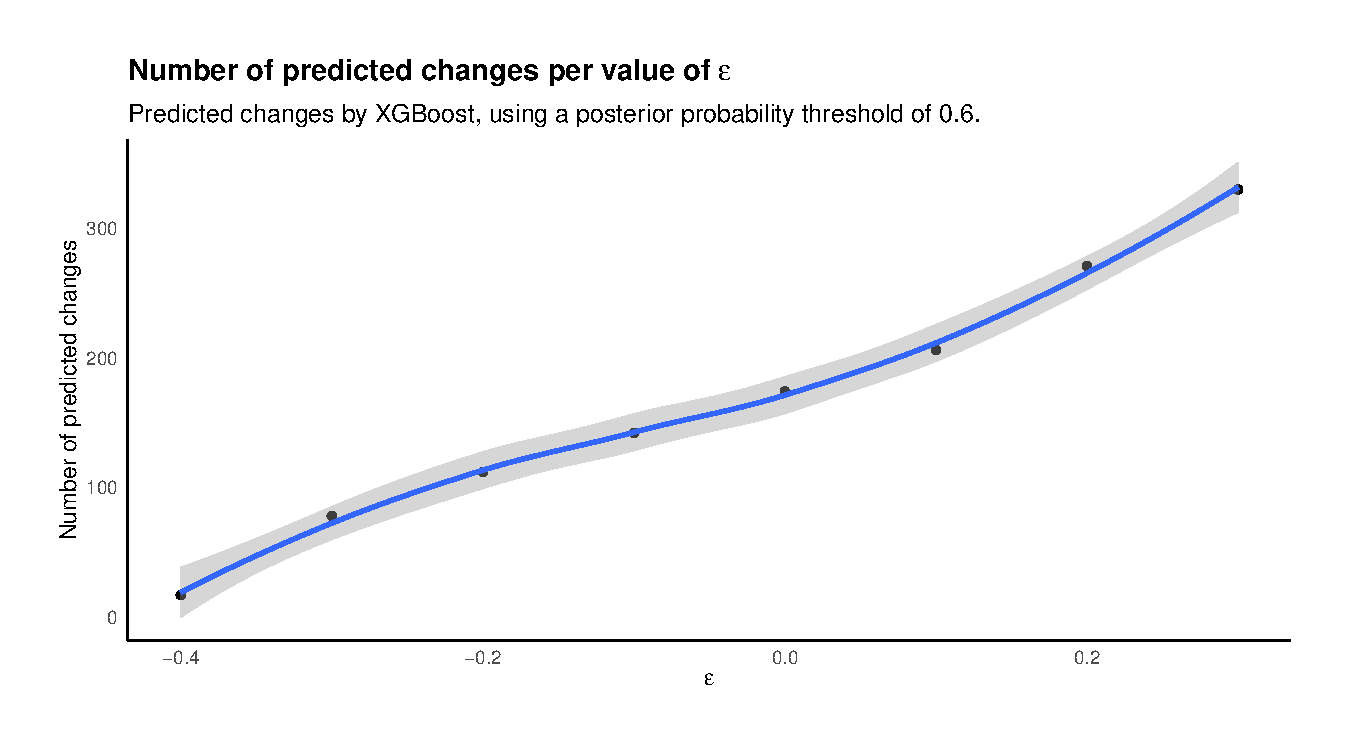
\includegraphics[width=\appfigwidth]{images/beta_plot.pdf}
    \caption{\textbf{Conditional-threshold calibration.}
    Predicted index changes as the conditional-threshold parameter $\varepsilon$ varies.
    The diagnostic shows why $\varepsilon=0.2$ is a pragmatic compromise: it materially increases signal count without pushing the strategy toward indiscriminate turnover.}
    \label{fig:app_beta}
\end{figure}

\begin{figure}[H]
    \centering
    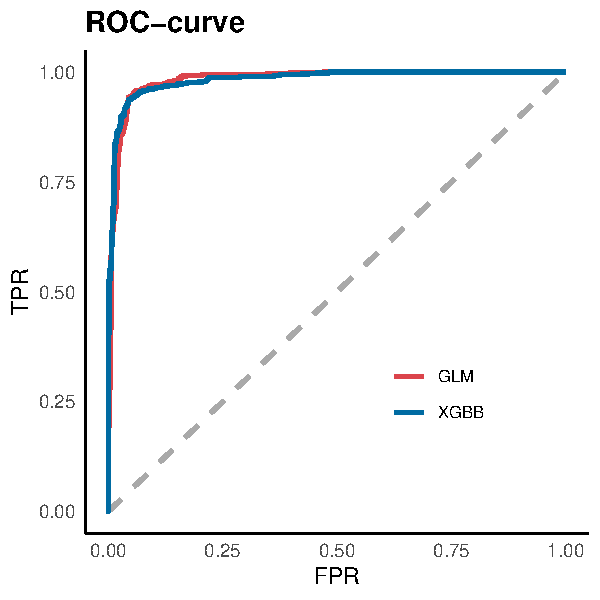
\includegraphics[width=0.5\textwidth]{images/roc_curve.pdf}
    \caption{\textbf{ROC curves for benchmark forecasts.}
    ROC curves for the 30-day GLM and XGBoost forecasts.
    The curve confirms that the underlying probability rankings remain informative before the announcement date, even when the final trading rule must still handle class imbalance and signal scarcity.}
    \label{fig:app_roc}
\end{figure}

\begin{figure}[H]
    \centering
    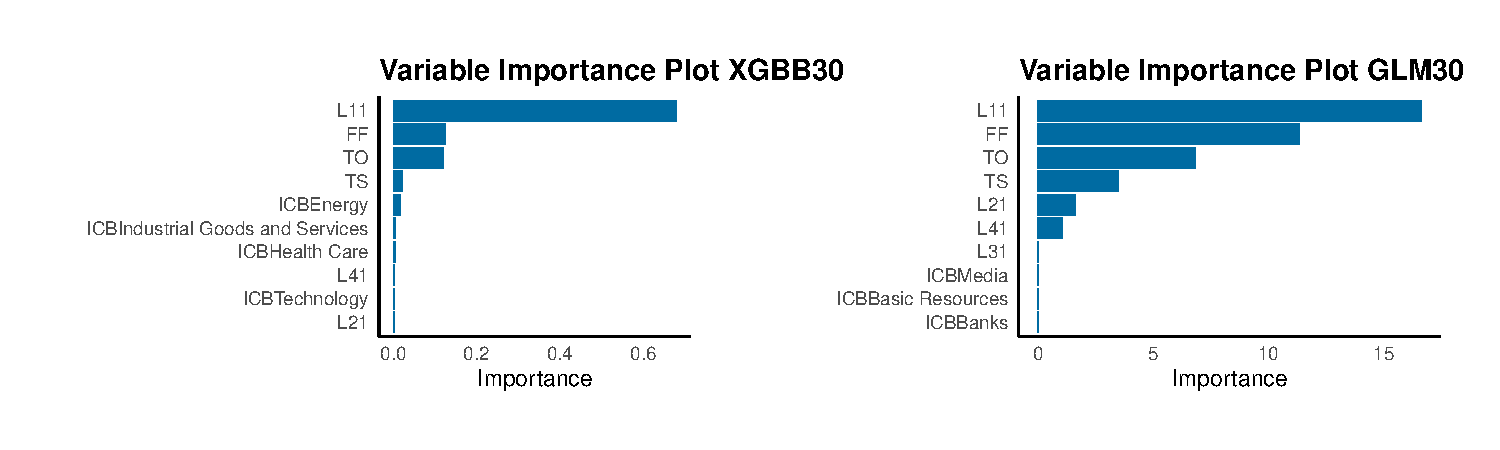
\includegraphics[width=\textwidth]{images/vip.pdf}
    \caption{\textbf{Variable importance for 30-day forecasts.}
    Lagged index membership dominates both models, while free float, turnover, trading status, and sector classification supply the marginal information needed to identify additions and deletions.}
    \label{fig:app_vip}
\end{figure}

\begin{figure}[H]
    \centering
    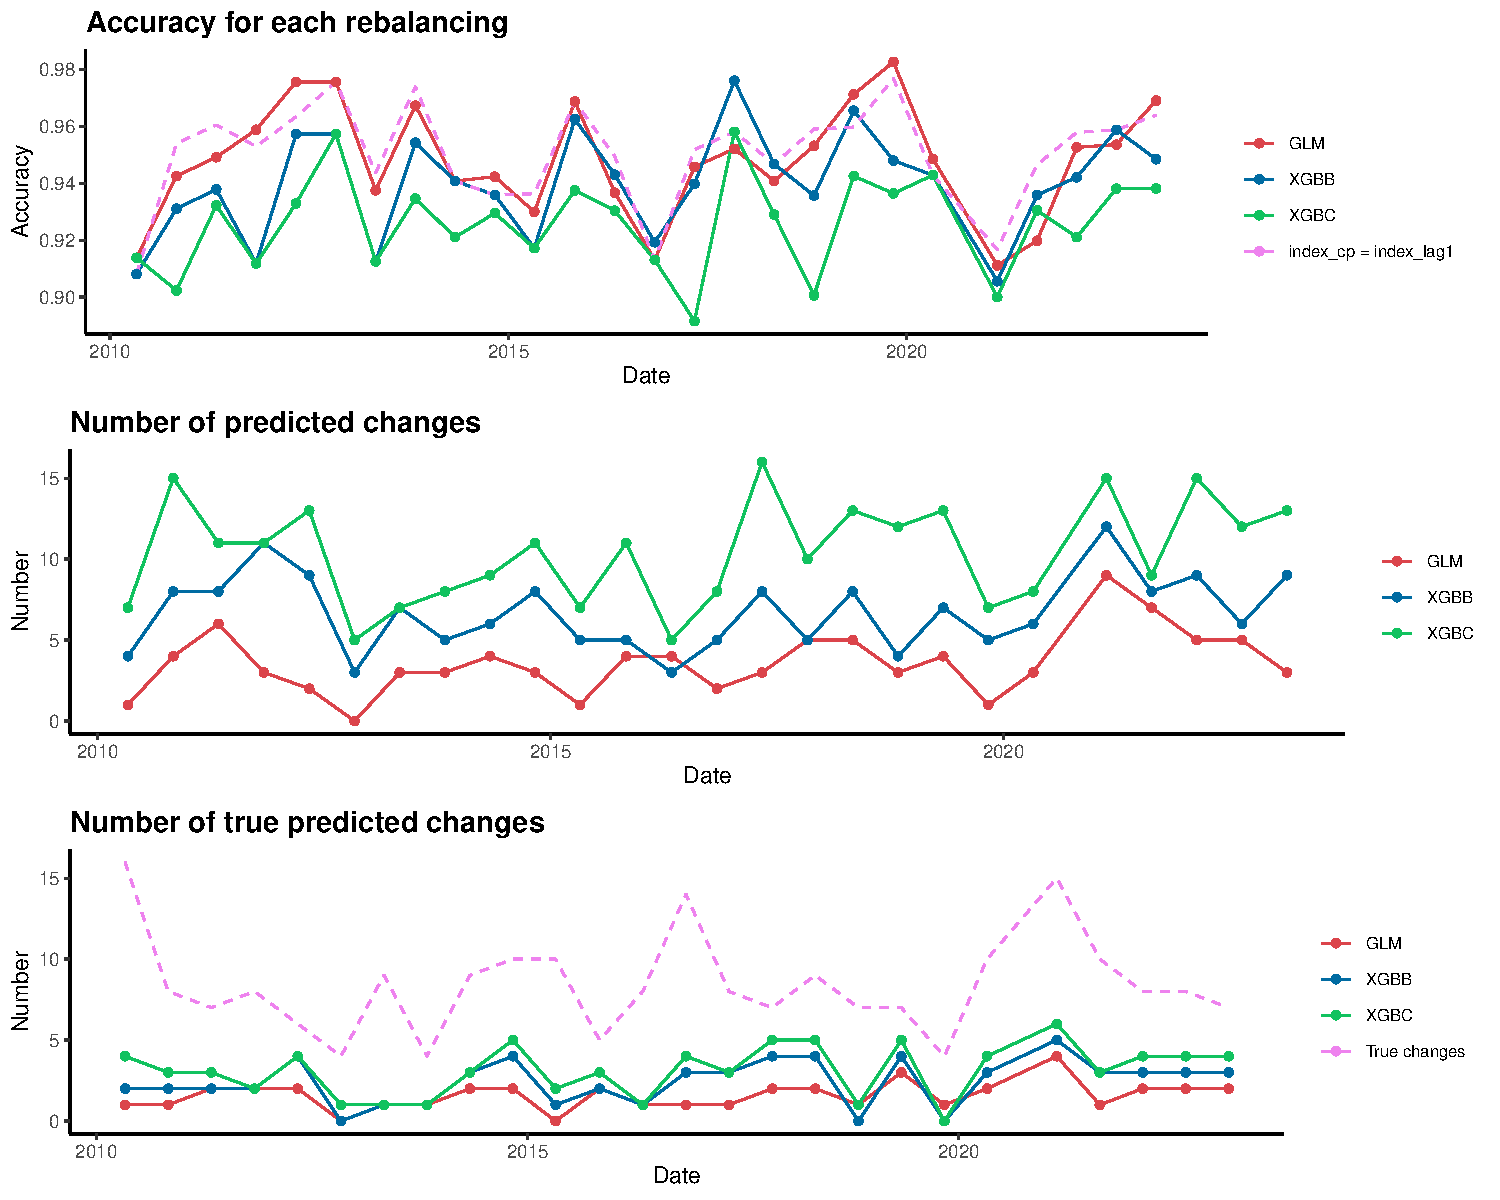
\includegraphics[width=\appfigwidth]{images/machinelearning_res.pdf}
    \caption{\textbf{Prediction performance through time.}
    Period-by-period accuracy, predicted changes, and captured changes for the 30-day GLM, XGBB, and XGBC specifications.
    The figure highlights the recurring trade-off between maximum classification accuracy and economically useful signal density.}
    \label{fig:app_ml_time}
\end{figure}

\begin{figure}[H]
    \centering
    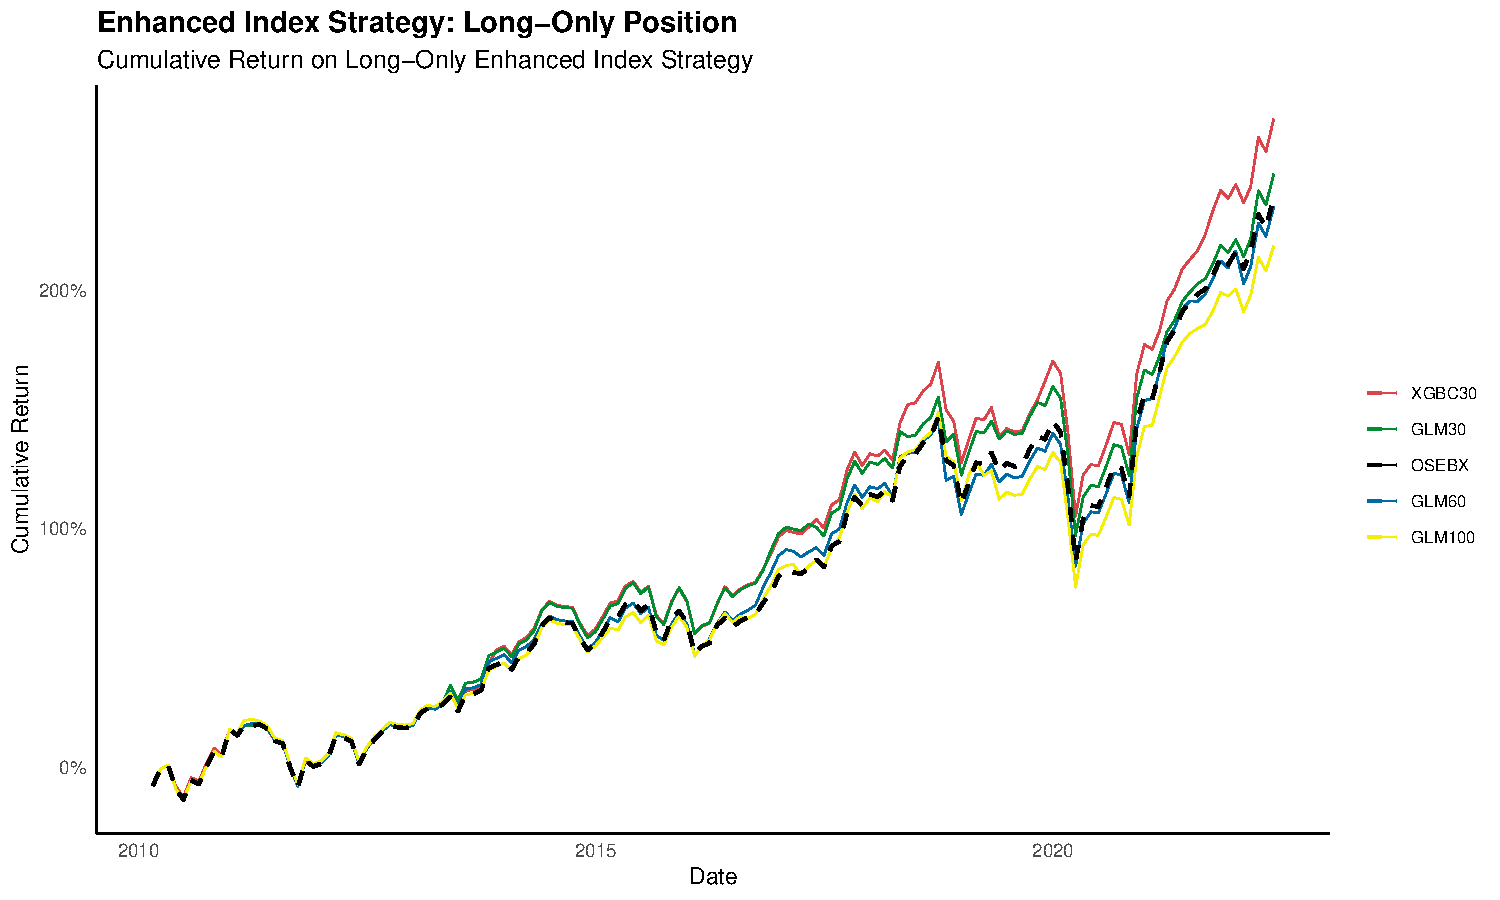
\includegraphics[width=\appfigwidth]{images/enhanced_long_only.pdf}
    \caption{\textbf{Long-only enhanced-index robustness check.}
    Long-only overlays also track OSEBX closely after scaling to the 2\% tracking-error budget, but none generates significant FF3 alpha in the thesis backtest.
    This supports the paper's focus on the long--short XGBC-30 variant.}
    \label{fig:app_enhanced_long_only}
\end{figure}